%==============================================================================
%== template for LATEX poster =================================================
%==============================================================================
%
%--A0 beamer slide-------------------------------------------------------------
\documentclass[final]{beamer}
\usepackage[orientation=landscape,size=a0,
            scale=1.25         % font scale factor
           ]{beamerposter}
           
\geometry{
  hmargin=2.5cm, % little modification of margins
}

%
\usepackage[utf8]{inputenc}

\linespread{1.15}
%
%==The poster style============================================================
\usetheme{sharelatex}

%==Title, date and authors of the poster=======================================
\title
[BAPG, 6 December 2014, Davis, CA, USA] % Conference
{ % Poster title
ANGSD-wrapper: a set of scripts to streamline NGS population genetics analysis
}

\author{ % Authors
Arun Durvasula\inst{1}, Tyler Kent\inst{1}, Siddharth Bhadra-Lobo\inst{1}, Jeffrey Ross-Ibarra\inst{2}
}
\institute
[University of California, Davis] % General University
{
\inst{1} Dept. of Plant Sciences, University of California Davis\\[0.3ex]
\inst{2} Dept. of Plant Sciences, Center for Population Biology, and Genome Center, University of California Davis\\[0.3ex]
}
\date{\today}



\begin{document}
\begin{frame}[t]
%==============================================================================
\begin{multicols}{3}
%==============================================================================
%==The poster content==========================================================
%==============================================================================

\section{Introduction}

	The advent of highly multiplexed sequencing has brought led to the rapid generation of new genomic data. One of the powerful approaches enabled by inexpensive sequencing is the ability to sequence a large number of individuals, each to relatively low sequencing depth. However this approach also presents statistical challenges in the analysis of low-coverage data.  The software package ANGSD (Korneliussen et al. 2014)In order to aid in the analysis of next generation sequencing data, population genetics software such as ANGSD has been developed. This program allows the user to calculate population genetic statistics such as site frequency spectrums, neutrality tests, and 
theta estimators from sequence data aligned to a reference. ANGSD uses likelihood based approaches to make full use of the data afforded by highly multiplexed sequencing. This has been used several studies to calculate summary statistics ( CITATIONS ). However, ANGSD requires much familiarity with command line tools and remains inaccessible to biologists that are not from a computational background. 
	Here we present a software package that aids in the preparation of analysis and facilitates analysis with interactive graphing software implemented in R and Shiny. Before analysis, angsd-wrapper turns a multistep analysis such as calculating Tajima’s D into one step where the information needed is supplied using a configuration file. After ANGSD has finished the calculations, a browser based application can be used to interactively graph the results. 


%\structure{Your text with scientific results or something...} $\hat H \Psi = E \Psi$  
%Your text with scientific results or something... 
%Your text with scientific results or something... 
%Your text with scientific results or something... 
%Your text with scientific results or something... 
%Your text with scientific results or something... 
%Your text with scientific results or something... 
%Your text with scientific results or something... 
%Your text with scientific results or something... 
%Your text with scientific results or something...
%
%\begin{equation}
%H = \sum_{i=1}^{N} h_{D}(i) + \sum_{j>i=1}^{N} C_{ij}
%\end{equation}
%
%Your text with scientific results or something... 
%Your text with scientific results or something... 
%Your text with scientific results or something... 
%Your text with scientific results or something... 
%Your text with scientific results or something... 
%Your text with scientific results or something... 
%Your text with scientific results or something... 
%Your text with scientific results or something... 
%Your text with scientific results or something... 
%Your text with scientific results or something... 
%Your text with scientific results or something... 
%Your text with scientific results or something... 
%Your text with scientific results or something... 
%Your text with scientific results or something... 
%Your text with scientific results or something... 
%Your text with scientific results or something... 
%Your text with scientific results or something... 
%Your text with scientific results or something... 
%Your text with scientific results or something... 
%Your text with scientific results or something...

In Ref.~\cite{ref1}...
In Refs.~\cite{ref1,ref2}...
On webpage~\cite{https://github.com/arundurvasula/angsd-wrapper}


\section{Implementation}

angsd-wrapper is implemented using several bash scripts that call ANGSD methods and handle saving intermediate files between the initial data preparation and the final data analysis. Each overall method in ANGSD, such as calculating estimates of ?, follows a specific order of program calls. Thus, we have abstracted away the running of each step and provided a set of default values for parameters and instead require the user to supply the data using a configuration file (figure 1a). The user can override the default values of the parameters in the configuration file as well.

Additionally, angsd-wrapper contains a powerful graphing application based on R and Shiny (figure 1b). After the analysis is done by ANGSD, the user can load the resulting statistics into a web-based application hosted on the user?s computer. This application allows the interactive plotting of values such as estimators of ? and Tajima?s D as well as the ability to load gene annotations from Ensembl. These features make it easy and intuitive to analyze next generation sequencing data. 
 


\vskip1ex
\begin{table}
\centering
\caption{This is a table with scientific results.}
\begin{tabular}{ccccc}
\hline\hline
1 & 2 & 3 & 4 & 5\\
\hline
aaa & bbb & ccc & ddd & eee\\
aaaa & bbbb & cccc & dddd & eeee\\
aaaaa & bbbbb & ccccc & ddddd & eeeee\\
aaaaaa & bbbbbb & cccccc & dddddd & eeeeee\\
1.000 & 2.000 & 3.000 & 4.000 & 5.000\\
\hline\hline
\end{tabular}
\end{table}
\vskip2ex

Your text with scientific results or something... 
Your text with scientific results or something... 
Your text with scientific results or something... 
Your text with scientific results or something... 
Your text with scientific results or something... 
Your text with scientific results or something... 
Your text with scientific results or something... 
Your text with scientific results or something... 
Your text with scientific results or something... 
Your text with scientific results or something... 
Your text with scientific results or something... 
Your text with scientific results or something... 
Your text with scientific results or something... 
Your text with scientific results or something... 
Your text with scientific results or something... 
Your text with scientific results or something... 
Your text with scientific results or something... 
Your text with scientific results or something... 
Your text with scientific results or something... 
Your text with scientific results or something... 


\subsection{SubSection}

Your text with scientific results or something... 
Your text with scientific results or something... 
Your text with scientific results or something... 
Your text with scientific results or something... 
Your text with scientific results or something... 
Your text with scientific results or something... 
Your text with scientific results or something... 
Your text with scientific results or something... 
Your text with scientific results or something... 
Your text with scientific results or something... 


\vskip1ex
\begin{figure}
\centering
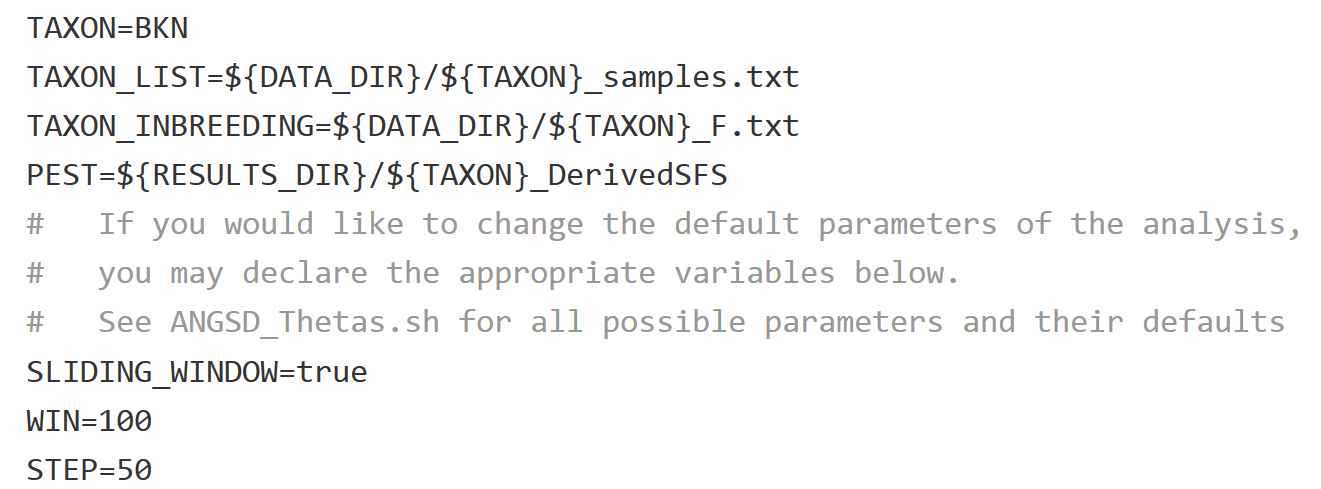
\includegraphics[width=0.99\columnwidth]{conf.png}
\caption{Figure 1a. Example configuration file.}
\end{figure}
\begin{figure}
\centering
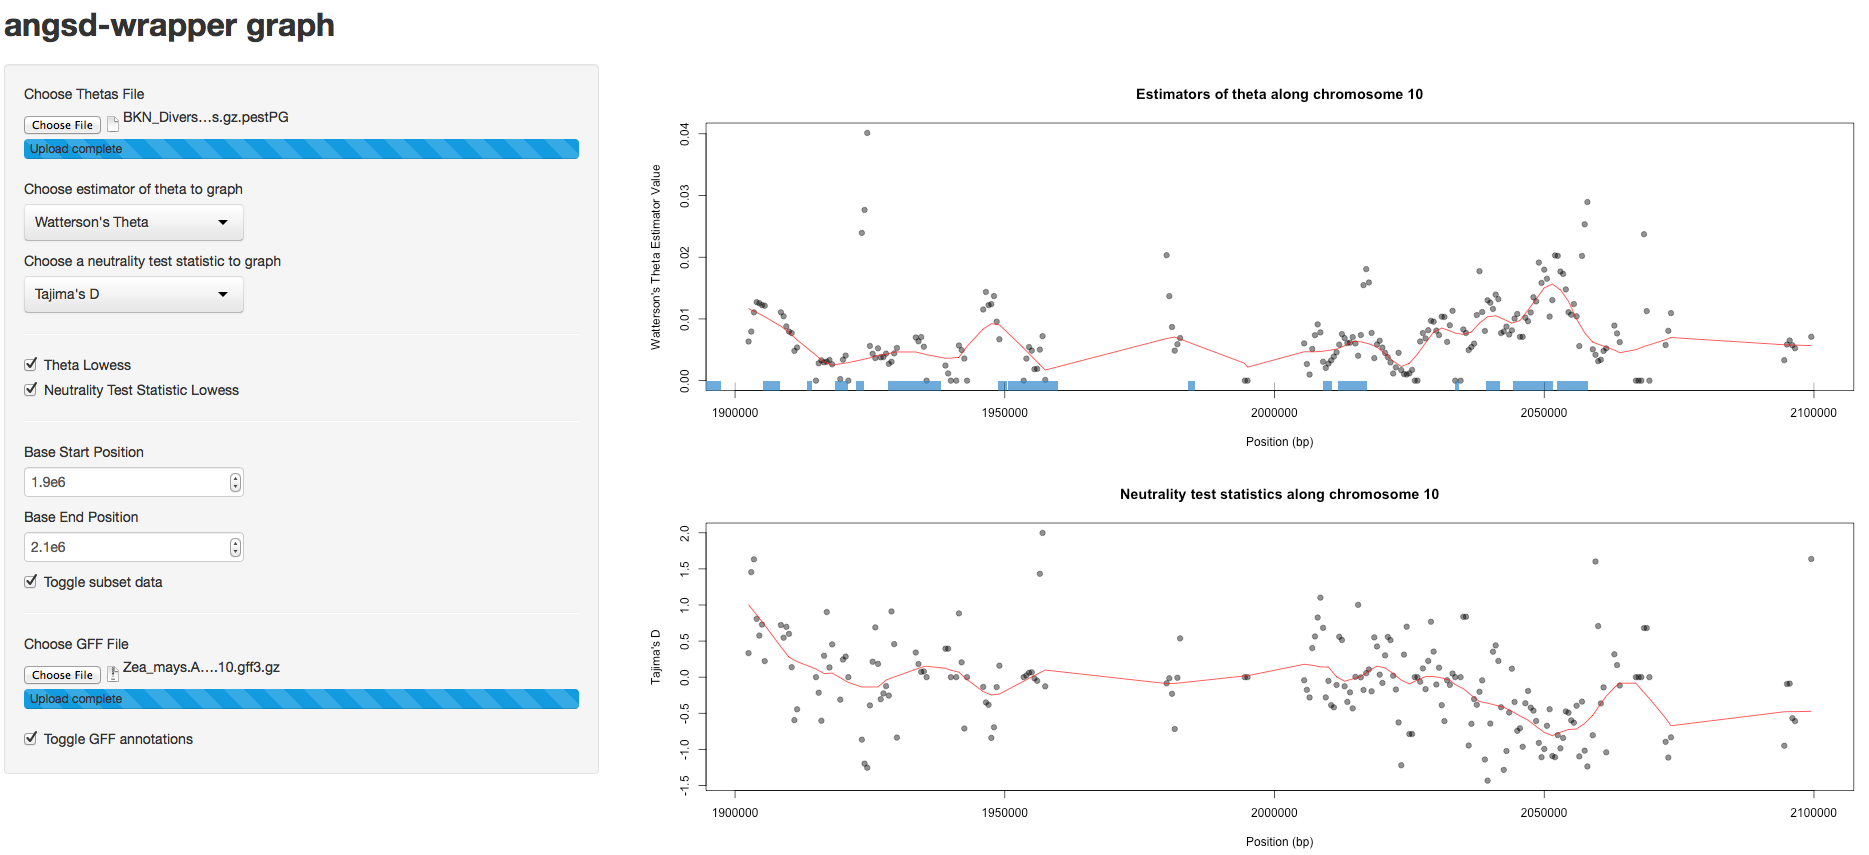
\includegraphics[width=0.99\columnwidth]{screenshot.png}
\caption{Figure 1b. angsd-wrapper interface}
\end{figure}
\vskip2ex

Your text with scientific results or something... 
Your text with scientific results or something... 
Your text with scientific results or something... 
Your text with scientific results or something... 
Your text with scientific results or something... 
Your text with scientific results or something... 
Your text with scientific results or something... 
Your text with scientific results or something... 
Your text with scientific results or something... 
Your text with scientific results or something... 
Your text with scientific results or something... 
Your text with scientific results or something... 
Your text with scientific results or something... 
Your text with scientific results or something... 
Your text with scientific results or something... 
Your text with scientific results or something... 
Your text with scientific results or something... 
Your text with scientific results or something... 
Your text with scientific results or something... 
Your text with scientific results or something...


\subsection{SubSection, a very very very very very very long title}

Your text with scientific results or something... 
Your text with scientific results or something... 
Your text with scientific results or something... 
Your text with scientific results or something... 
Your text with scientific results or something... 
Your text with scientific results or something... 
Your text with scientific results or something... 
Your text with scientific results or something... 
Your text with scientific results or something... 
Your text with scientific results or something... 
Your text with scientific results or something... 
Your text with scientific results or something... 
Your text with scientific results or something... 
Your text with scientific results or something... 
Your text with scientific results or something... 
Your text with scientific results or something... 
Your text with scientific results or something... 
Your text with scientific results or something... 
Your text with scientific results or something... 
Your text with scientific results or something...

\section{Summary and conclusions}

Your text with scientific results or something... 
Your text with scientific results or something... 
Your text with scientific results or something... 
Your text with scientific results or something... 
Your text with scientific results or something... 
Your text with scientific results or something... 
Your text with scientific results or something... 
Your text with scientific results or something... 
Your text with scientific results or something... 
Your text with scientific results or something... 

Your text with scientific results or something... 
Your text with scientific results or something... 
Your text with scientific results or something... 
Your text with scientific results or something... 
Your text with scientific results or something... 
Your text with scientific results or something... 
Your text with scientific results or something... 
Your text with scientific results or something... 
Your text with scientific results or something... 
Your text with scientific results or something... 


%==============================================================================
%==End of content==============================================================
%==============================================================================

%--References------------------------------------------------------------------

\subsection{References}

\begin{thebibliography}{99}

\bibitem{ref1} J.~Doe, Article name, \textit{Phys. Rev. Lett.}

\bibitem{ref2} J.~Doe, J. Smith, Other article name, \textit{Phys. Rev. Lett.}

\bibitem{web} \url{http://www.google.pl}

\end{thebibliography}
%--End of references-----------------------------------------------------------

\end{multicols}

%==============================================================================
\end{frame}
\end{document}
